\begin{figure}[H]
    \centering
    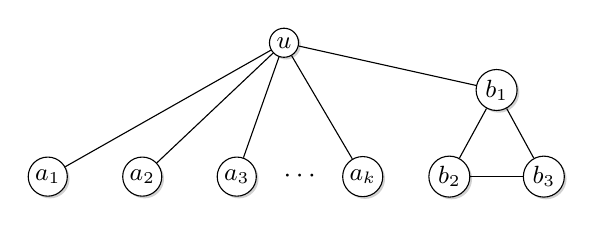
\begin{tikzpicture}[vtx/.style={circle,draw,fill=white,inner sep=1.4pt,font=\small,preaction={fill=black,opacity=0.18,transform canvas={xshift=0.8pt,yshift=-0.8pt}}}]
        \node[vtx] (u) at (0.8,0) {$u$};
        \node[vtx] (a1) at (-2.2,-1.7) {$a_1$};
        \node[vtx] (a2) at (-1.0,-1.7) {$a_2$};
        \node[vtx] (a3) at (0.2,-1.7) {$a_3$};
        \node[vtx] (ak) at (1.8,-1.7) {$a_k$};
        \node (dots) [draw=none,fill=none,preaction={},shape=rectangle,inner sep=0pt,outer sep=0pt,minimum size=0pt] at (1.0,-1.7) {$\cdots$};

        \node[vtx] (b1) at (3.5,-0.6) {$b_1$};
        \node[vtx] (b2) at (2.9,-1.7) {$b_2$};
        \node[vtx] (b3) at (4.1,-1.7) {$b_3$};

        \draw (u) -- (a1);
        \draw (u) -- (a2);
        \draw (u) -- (a3);
        \draw (u) -- (ak);
        \draw (u) -- (b1);

        \draw (b1) -- (b2);
        \draw (b2) -- (b3);
        \draw (b3) -- (b1);
    \end{tikzpicture}
    \caption{Example of graph for which the multiplicative difference between values of both clustering objective functions is $\Theta\br{n}$.}
    \label{fig:star-triangle-example}
\end{figure}
